\chapter*{Appendix A: Feature importance on Shapley plots}
\label{appendix:A}

\renewcommand{\thefigure}{A.\arabic{figure}} 
\setcounter{figure}{0} % Reset figure counter

\begin{figure}[H]
    \centering
    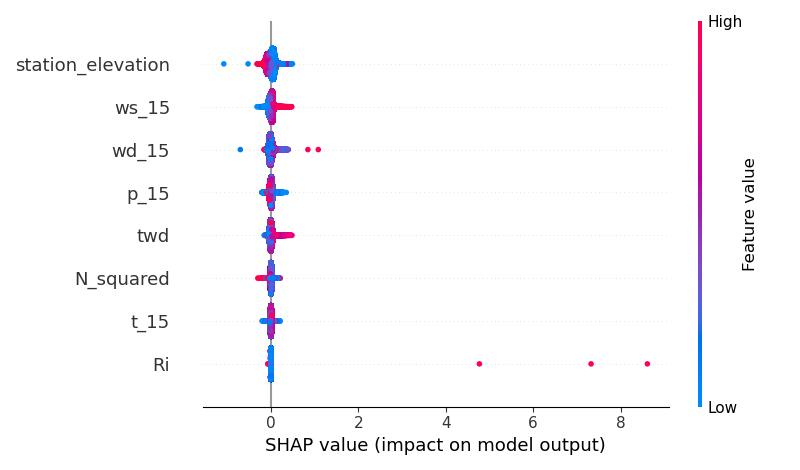
\includegraphics[scale = 0.6]{Figures/shap_plots/summary_plot_190924_full_10ms.png}
    \caption[Summary feature importance of a neural network using entire dataset.]{Feature importance of a neural network with model architecture as described in Table \ref{table:gridSearchHyperparameters} and data as described in Table \ref{table:trainDataExample}. The distribution seems to be the same as before, discounting the outliers.}
    \label{fig:ShapleySummary3}
\end{figure}

\begin{figure}[H]
    \centering
    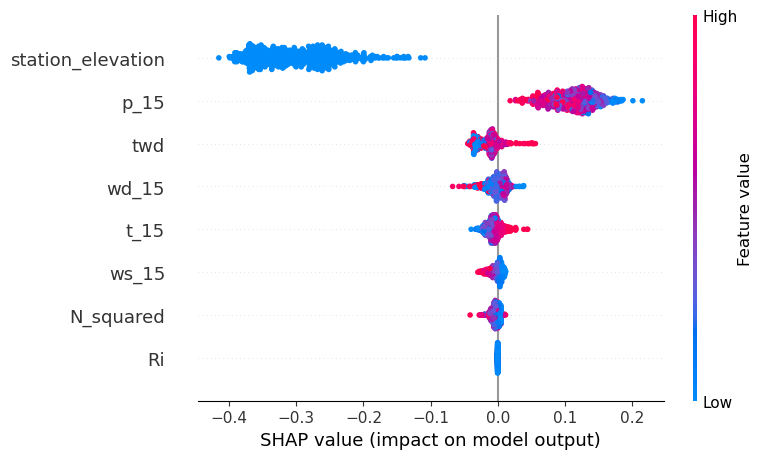
\includegraphics[scale = 0.6]{Figures/shap_plots/summary_plot_6745.png}
    \caption[Summary feature importance of a neural network only looking at AWS at Ásgarðsfjall.]{Feature importance of a neural network with model architecture as described in Table \ref{table:gridSearchHyperparameters} and data as described in Table \ref{table:trainDataExample}. This plot only looks at datapoints from Ásgarðsfjall. This seems to show the same distribution as previous summary plots. Station elevation is influential and Richardson number has no impact.}
    \label{fig:ShapleySummaryAsgarðsfjall}
\end{figure}

\begin{figure}[H]
    \centering
    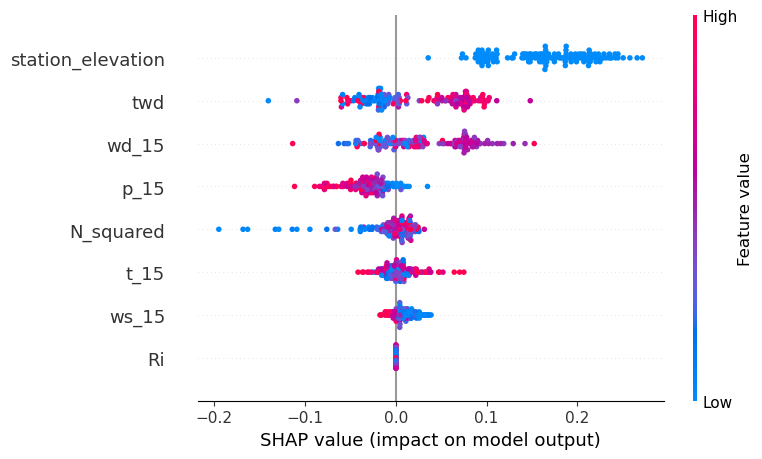
\includegraphics[scale = 0.6]{Figures/shap_plots/summary_plot_1470.png}
    \caption[Summary feature importance of a neural network only looking at AWS at Háahlíð.]{Feature importance of a neural network with model architecture as described in Table \ref{table:gridSearchHyperparameters} and data as described in Table \ref{table:trainDataExample}. This plot only looks at datapoints from Háahlíð. This seems to show the same distribution as previous summary plots. Station elevation is influential and Richardson number has no impact.}
    \label{fig:ShapleySummaryHaahlid}
\end{figure}